%!TEX TS-program = xelatex
\documentclass[]{friggeri-cv}
\usepackage{afterpage}
\usepackage{hyperref}
\usepackage{url}
\usepackage{color}
\usepackage{xcolor}
\hypersetup{
    pdftitle={herve-beraud-cv-en.pdf},
    pdfauthor={Hervé Beraud},
    pdfsubject={Hervé Beraud curriculum vitae},
    pdfkeywords={},
    colorlinks=false,       % no lik border color
    allbordercolors=white    % white border color for all
}
\addbibresource{bibliography.bib}
\RequirePackage{xcolor}
\definecolor{pblue}{HTML}{0395DE}

\begin{document}
\header{Hervé }{Beraud}
{DevOps architect}

% Fake text to add separator
\fcolorbox{white}{gray}{\parbox{\dimexpr\textwidth-2\fboxsep-2\fboxrule}{%
.....
}}

% In the aside, each new line forces a line break
\begin{aside}
    \section{Address}
        32450,~Castelnau~Barbarens
        France
        ~
    \section{Contact}
        +33.661.840.417
        \href{mailto:herveberaud.pro@gmail.com}{\textbf{herveberaud.pro@}\\gmail.com}
        ~
    \section{Social (click)}
        \href{https://github.com/4383}{github: 4383}
        \href{https://hub.docker.com/r/4383}{dockerhub: 4383}
        \href{https://warehouse.python.org/user/4383/}{pypi: 4383}
        \href{https://twitter.com/4383hberaud}{twitter: 4383hberaud}
        ~
    \section{Technologies}
        \textbf{Python}
\includegraphics[scale=0.40]{img/5stars.png}
        \textbf{Shell}
\includegraphics[scale=0.40]{img/4stars.png}
        \textbf{Ansible}
\includegraphics[scale=0.40]{img/4stars.png}
        \textbf{Git}
\includegraphics[scale=0.40]{img/5stars.png}
        \textbf{Docker}
\includegraphics[scale=0.40]{img/4stars.png}
        \textbf{CI/CD}
\includegraphics[scale=0.40]{img/5stars.png}
        ~
    \section{OS Preference}
        \textbf{GNU/Linux}
\includegraphics[scale=0.40]{img/5stars.png}
        \textbf{Unix}
\includegraphics[scale=0.40]{img/4stars.png}
        \textbf{MacOS}
\includegraphics[scale=0.40]{img/2stars.png}
        \textbf{Windows}
\includegraphics[scale=0.40]{img/1stars.png}
        ~
    \section{Methodologies}
        \textbf{Agile}
\includegraphics[scale=0.40]{img/5stars.png}
        \textbf{Lean}
\includegraphics[scale=0.40]{img/4stars.png}
        \textbf{Kanban}
\includegraphics[scale=0.40]{img/4stars.png}
        ~
\end{aside}

\section{Personal Philosophy}
    Time is a store of value much higher than any precious currency or material. Throughout our lives time acquires with money, we buy time.
    My job as DevOps is to automate and industrialize processes, so generate time and therefore value.

\section{Education}
\begin{entrylist}
    \entry
        {2010 - now}
        {Engineer Degree in Computer Science}
        {CNAM Aix en Provence, France}
        {Curriculum information systems.\\
        Main subjects: Systems \& Software Architecture and Security, Urbanism for Evolving Systems.\\}
    \entry
        {2009 - 2010}
        {BTEC Higher National Diploma in Software Development}
        {AFPA Istres, France}
        {Main subjects: Software Architecture, Modeling Tools (Merise, UML).\\}
    \entry
        {1999 - 2001}
        {BTEC National Diploma in Landscape Architect}
        {Lycée Fontlongue Miramas, France}
        {Agricultural college.\\
        Main subjects: Design and Advise on the Construction of Urban, Rural, Residential and Public Landscape.\\}
    \entry
        {1999 - 2001}
        {BTEC First Diploma in Nursery Gardener}
        {Lycée Fontlongue Miramas, France}
        {Agricultural college.\\
        Main subjects: Cultivating, Harvesting, Transplanting Trees, Shrubs or Plants.}
\end{entrylist}

\section{Awards}
\begin{entrylist}
  \entry
    {2016}
    {Winner of squad incubator contest}
    {French annual IT innovation contest}
    {\emph{Design a DevOps solution for automatizing security scanning on web apps CI/CD workflow and project lifecycle}}
\end{entrylist}

\section{Contributions to open source projects}
\begin{entrylist}
  \entry
    {provisioning}
    {\href{https://github.com/ansible/ansible}{ansible}}
    {community contributor}
    {\emph{bugfix, code cleaning, implement tests}}
  \entry
    {system}
    {\href{https://github.com/alpinelinux/aports}{alpine linux - aports}}
    {community contributor}
    {\emph{package maintaining, proposal new testing packages}}
  \entry
    {workflow}
    {\href{https://github.com/jd/git-pull-request}{github-pull-request}}
    {community contributor}
    {\emph{implement new feature}}
  \entry
    {development}
    {\href{https://github.com/AntoineCezar/cookiecutter-pypkg}{cookiecutter-pypkg}}
    {core maintainer}
    {\emph{implement new features, bugfix, reviewer, project workflow management}}
\end{entrylist}


\newpage
\section{Experience}
\begin{entrylist}
    \entry
        {03-16 - Now}
        {Lead cloud DevOps architect}
        {Orange OINIS ITE, Toulouse, France}
        {Architect, design, and deliver technical solutions for automatizing deployment of openstack tripleO infrastructure. Design products and continuous deployment system and infrastructure automation strategy.\\}
    \entry
        {09-16 - 03-17}
        {DevOps architect | Python lead developer}
        {Squad / CNES, Toulouse, France}
        {Architect, design, develop and deliver european space program ISIS guidance system. Manage project workflow.\\}
    \entry
        {05-16 - Now}
        {DevOps Technical Leader}
        {Squad (internal), Toulouse, France}
        {Team Technical management, manage DevOps community, animate technical events, create design and setup the squad official software forge. Apply security ehancements and best practices.\\}
    \entry
        {04-14 - 04-16}
        {DevOps architect}
        {BULL / EDF, Toulouse, France}
        {Design and develop algorithms, solutions for call center and workload management system. Design and develop multi-channel agent desktop.
        Create and develop Python/Django webapps for generating, deploye, and maintaince version for C\# project (automatized continuouse integration).\\}
    \entry
        {09-13 - 03-14}
        {Embedded Software Engineer}
        {BULL / French Navy, Aix en Provence, France}
        {Design continuous integration, design system architecture , AIX5.3 and Unix software.\\}
    \entry
        {02-13 - 09-13}
        {Software Engineer}
        {BULL / DCNS, Toulon, France}
        {Design and develop electronic warefare system on the FREMM frigate project.\\}
    \entry
        {06-11 - 01-13}
        {Frontend / Backend Web Developer}
        {BULL / Virtual-expo, Marseille, France}
        {Design and development of a world expert online exhibitions website on Linux/Apache/PHP/Zend platform. Design, development of a Python web crawler.\\}
    \entry
        {04-11 - 06-11}
        {System Administrator / Backend Developer}
        {Distrimag, Arles, France}
        {Maintain data center environmental and monitoring equipment (IBM AS400). Virtualize physical server. PHP Development of stock managment software.\\}
    \entry
        {10-10 - 03-11}
        {Frontend Web / Backend Developer}
        {PlusValue SAS, Vitrolles, France}
        {Management and migration of servers. Development of php web micro-framework. Development of web templates and interfaces. Management of SQL databases.\\}
    \entry
        {12-04 - 01-09}
        {Buisness Owner}
        {Damofli Fruits \& Legumes, France}
        {Manage marketing operations, accounting, sales plans, inventory management.\\}
    \entry
        {09-01 - 11-04}
        {Landscape Architect}
        {Local Council of Martigues, France}
        {Manage marketing operations, accounting, sales plans, inventory management.\\}
\end{entrylist}

\begin{aside}
~
~
~
    \section{Character}
        Passionate
        Self-educated
        Autonomous
        Curious
        Pragmatic
        ~
    \section{Personal Skills}
        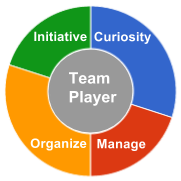
\includegraphics[scale=0.62]{img/personal.png}
        ~
\end{aside}

\newpage

\section{Personal projects}
\begin{entrylist}
  \entry
    {2016}
    {\href{https://github.com/gr0und-s3ct0r/apkbuild}{Apkbuild - Dockerized build environment for apk (click to see)}}
    {Personal project}
    {\emph{Docker, Docker hub, Ubuntu, Vim, etc...}}
  \entry
    {2016}
    {\href{https://github.com/4383/machine}{Machine - Dockerized Development Environment (click to see)}}
    {Personal project}
    {\emph{Docker, Docker hub, Ubuntu, Vim, etc...}}
  \entry
    {2016}
    {\href{https://github.com/4383/Botanick}{Botanick - web application for collect emails (click to see)}}
    {Personal project}
    {\emph{Docker, Python, Flask, Git, Github, Travis-CI, Docker hub}}
  \entry
    {2016}
    {\href{https://github.com/mhackgyver-squad/porno-king}{Port Knocking Sequence Discovery Scanner (click to see)}}
    {Personal project}
    {\emph{Docker, Python, Git, Github, Docker hub}}
  \entry
    {2016}
    {\href{https://github.com/mhackgyver-squad/mhackgyver}{Mhackgyver official repository (click to see)}}
    {Professional project}
    {\emph{Create and maintain tools for mhackgyver pentest team}}
  \entry
    {2016}
    {\href{https://hub.docker.com/r/4383/discosub}{Discosub Dockerized Security Scanner (click to see)}}
    {Personal project}
    {\emph{Docker, Python, Docker hub, Travis-CI, Pypi, Github, Git, tor, ubuntu}}
  \entry
    {2016}
    {\href{https://hub.docker.com/r/4383/system-service-footprint}{Nmap Dockerized Security Scanner (click to see)}}
    {Personal project}
    {\emph{Docker, Docker hub, Github, Git, nmap, tor, ubuntu}}
  \entry
    {2016}
    {\href{https://hub.docker.com/r/4383/director}{Director Dockerized Security Scanner (click to see)}}
    {Personal project}
    {\emph{Docker, Docker hub, Github, Git, dirb, tor, ubuntu}}
  \entry
    {2016}
    {\href{https://hub.docker.com/r/4383/irc-server}{Dockerized IRC server (click to see)}}
    {Personal project}
    {\emph{Docker, Docker hub, Github, Git, ircd-irc2, ubuntu}}
  \entry
    {2015}
    {\href{http://pypi.python.org/pypi/barcode-generator/0.1rc15}{Barcode Generator (click to see)}}
    {Personal project}
    {\emph{Python 3 / SVG / Git}}
  \entry
    {2015}
    {\href{https://github.com/4383/street-workout-database}{The Street Workout Database (offline)}}
    {Personal project}
    {\emph{Python / Django / Javascript / JQuery/ HTML5 / Bootstrap / Debian 7 / PostGreSQL / Nginx / Supervisor / Git}}
  \entry
    {2013}
    {\href{https://github.com/4383/fabric-debian/}{Security Best Practices Automatic Setup (click to see)}}
    {Personal project}
    {\emph{Python / Iptables /  debian 6 / port-knocking / Fail2Ban / PostGreSQL / Nginx}}
\end{entrylist}


\begin{aside}
~
~
~
  \section{I Like It}
    
\includegraphics[scale=0.18]{img/python.png}
    
\includegraphics[scale=0.18]{img/docker.png}
    
\includegraphics[scale=0.18]{img/arch.png}
    
\includegraphics[scale=0.06]{img/vim.png}
    
\includegraphics[scale=0.06]{img/latex.png}
    
\includegraphics[scale=0.08]{img/gnu.png}
    \href{http://www.herve-beraud.ovh/skills/}{And More...}
    ~
  \section{About me}
    Year of birth : 1982
    married, 4 childrens 
    ~
  \section{Languages}
    \textbf{French}
\includegraphics[scale=0.40]{img/5stars.png}
    \textbf{English}
\includegraphics[scale=0.40]{img/3stars.png}
\end{aside}

\section{Hobbies and Interests}
\begin {itemize}
    \item \emph {Sports (Street Workout, Swimming, Running)}
    \item \emph {Family}
    \item \emph {Member of mhackgyver pentest team, participate to cybersecurity challenges}
    \item \emph {Computer Sciences (ArchLinux, Python, Arduino, Vim)}
    \item \emph {Psychology / Philosophy (Carl Jung, neuro linguistic programing, etc...)}
    \item \emph {Traveling (Senegal, Ivory Coast, Europe)}
\end {itemize}

\begin{flushright}
\emph{Latest update - October, 2017}
\end{flushright}
\end{document}
